\section{Introducción}


\subsection{Presentación}
\begin{frame}{Introducción}{Presentación}
  \begin{figure}[h]
  \centering
  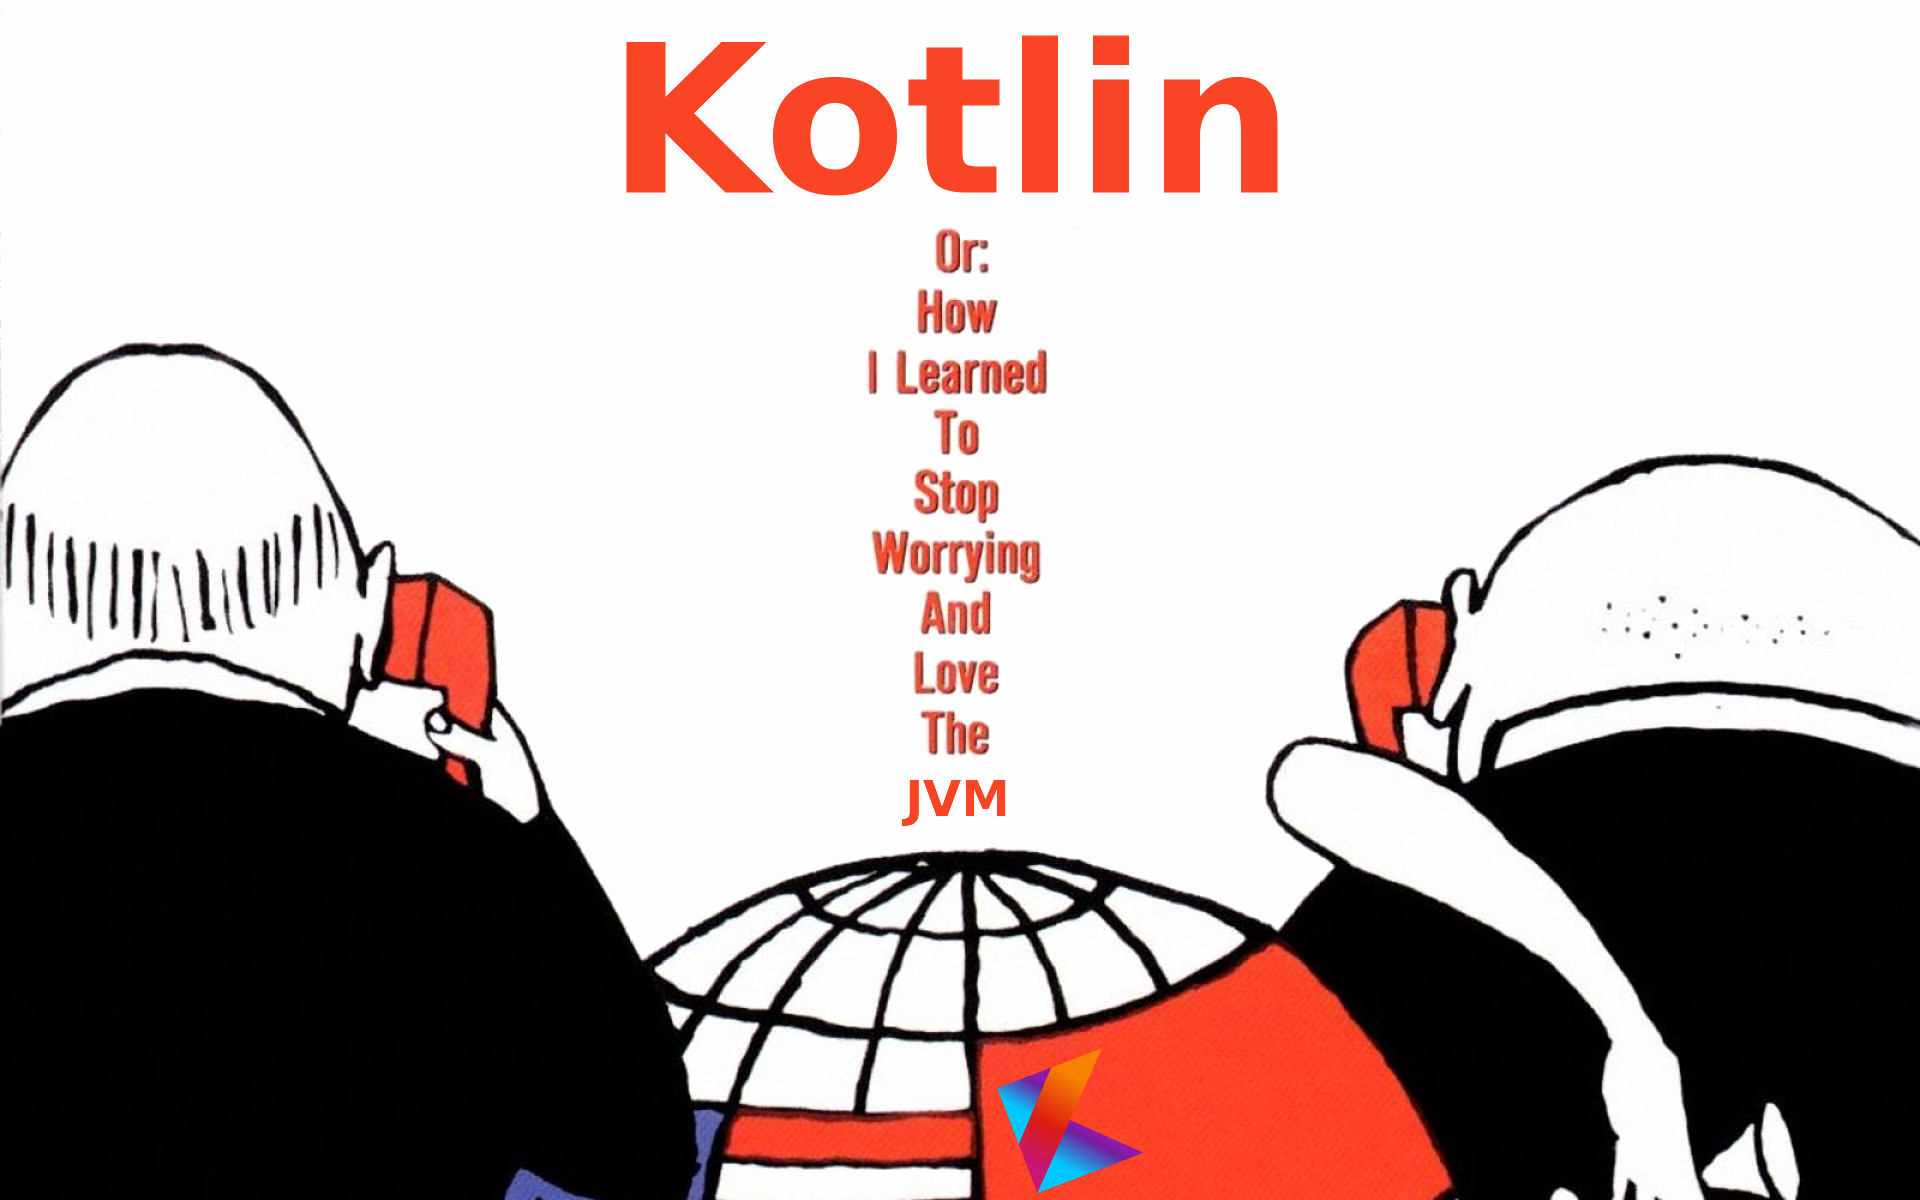
\includegraphics[width=\textwidth]{images/introduction/cover}
  \end{figure}
\end{frame}
%%%%%%%%%%%%%%%%

\begin{frame}{Introducción}{Presentación}
 \begin{block}{Pablo García Fernández}
  \vspace{\baselineskip}
  \minipage{0.25\textwidth}
  \begin{figure}[h]
   \centering
   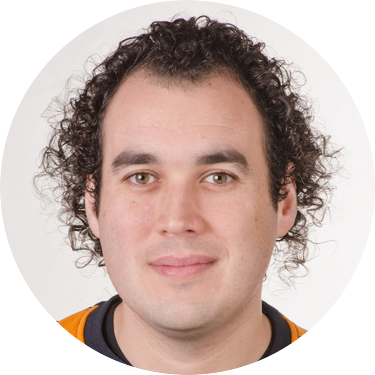
\includegraphics[width=\textwidth]{images/introduction/me_round}
  \end{figure}
  \endminipage
  \minipage{0.75\textwidth}
  \begin{itemize}
   \item Graduado en \textbf{Ingeniería del Software} (Universidad de Oviedo)
   \item \textbf{Associate Android Developer} (Google)
   \item Senior Software Engineer en \textbf{Sngular}
  \end{itemize}
  \endminipage\hfill
 \end{block}
 \begin{itemize}
  \item \href{mailto:pablogf.casia@gmail.com}{{\faEnvelope} pablogf.casia@gmail.com}
  \item \href{http://www.pablocasia.com/}{{\faDesktop} http://www.pablocasia.com/}
  \item \href{https://www.linkedin.com/in/pablocasia/}{{\faLinkedin} https://www.linkedin.com/in/pablocasia/}
  \item \href{https://github.com/PabloCasia}{{\faGithub} https://github.com/PabloCasia}
 \end{itemize}
\end{frame}
%%%%%%%%%%%%%%%%

\subsection{Historia}
\begin{frame}{Introducción}{Historia}
 \begin{itemize}
  \item<1-> El \textbf{19 de Julio del 2011} durante el \textbf{JVM Language Summit}, una conferencia de desarrolladores Java enfocada en la máquina virtual,
  \textbf{JetBrains} anunciaba que llevaba un año trabajando en un nuevo lenguaje para la JVM llamado \textbf{Kotlin}.
  \item<2-> El \textbf{14 de Febrero de 2012} el proyecto se hizo \textbf{Open Source} bajo licencia Apache 2.0.
 \end{itemize}
 \begin{figure}[!htb]
    \minipage{0.3\textwidth}
    \endminipage
    \minipage{0.3\textwidth}
    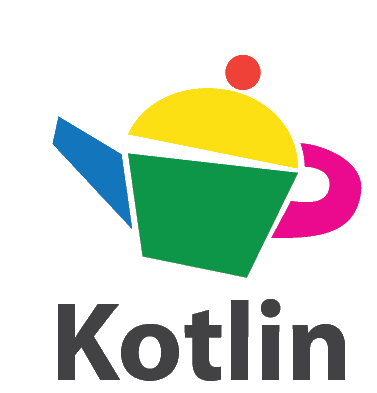
\includegraphics[width=\linewidth]{images/introduction/kotlin_logo_0}
    \endminipage
    \minipage{0.3\textwidth}
    \endminipage
   \end{figure}
\end{frame}
%%%%%%%%%%%%%%%%
\begin{frame}{Introducción}{Historia}
 \begin{itemize}
  \item El 19 de Julio del 2011 durante el JVM Language Summit se anuncia Kotlin.
  \item El 14 de Febrero de 2012 el proyecto se hizo Open Source bajo licencia Apache 2.0.
  \item<1-> El \textbf{26 de Agosto de 2013} fue lanzado el plugin para \textbf{Android Studio}.
  \item<2-> El \textbf{15 de Febrero de 2015} después de varias builds y betas se lanza \textbf{Kotlin 1.0}.
  \begin{figure}[!htb]
     \minipage{0.3\textwidth}
     \endminipage
     \minipage{0.3\textwidth}
     
\includegraphics[width=\linewidth]{images/introduction/kotlin_logo_1}
     \endminipage
     \minipage{0.3\textwidth}
     \endminipage
    \end{figure}
\end{itemize}
\end{frame}
%%%%%%%%%%%%%%%%
\begin{frame}{Introducción}{Historia}
 \begin{itemize}
  \item El 19 de Julio del 2011 se anuncia Kotlin.
  \item El 14 de Febrero de 2012 el proyecto se hizo Open Source.
  \item El 26 de Agosto de 2013 fue lanzado el plugin para Android Studio.
  \item El 15 de Febrero de 2015 se lanza Kotlin 1.0.
  \item El \textbf{1 de Marzo de 2017} se lanza \textbf{Kotlin 1.1} con soporte para la JVM, Android y JS.
 \end{itemize}
 \begin{figure}[!htb]
    \minipage{0.3\textwidth}
    \endminipage
    \minipage{0.3\textwidth}
    
\includegraphics[width=\linewidth]{images/introduction/kotlin_logo_2}
    \endminipage
    \minipage{0.3\textwidth}
    \endminipage
   \end{figure}
\end{frame}
%%%%%%%%%%%%%%%%
\begin{frame}{Introducción}{Historia}
 \begin{itemize}
   \item El 19 de Julio del 2011 se anuncia Kotlin.
   \item El 14 de Febrero de 2012 el proyecto se hizo Open Source.
   \item El 26 de Agosto de 2013 fue lanzado el plugin para Android Studio.
   \item El 15 de Febrero de 2015 se lanza Kotlin 1.0.
  \item El 1 de Marzo de 2017 se lanza Kotlin 1.1 con soporte para la JVM, Android y JS.
  \item El \textbf{17 de Mayo de 2017} durante la conferencia \textbf{Google I\/O} se anuncia el \textbf{soporte oficial}
  del lenguaje dentro de la plataforma \textbf{Android}.
 \end{itemize}
\end{frame}
%%%%%%%%%%%%%%%%
\subsection{¿Qué es Kotlin?}
\begin{frame}{Introducción}{¿Qué es Kotlin?}
 Kotlin es un \textbf{lenguaje de programación: }
 \begin{itemize}
  \item<1-> Desarrollado por \textbf{JetBrains}.
  \item<2-> Estaticamente tipado.
  \item<3-> 100\% interoperable con Java.
  \item<4->
  \begin{itemize}
    \item Java
    \item Android
    \item JavaScript
    \item Kotlin/Native
  \end{itemize}
 \end{itemize}
\end{frame}
%%%%%%%%%%%%%%%%
